\chapter{Methodoloy}\label{chap:methodology}



\section{Feature Selection}
\indent As mentioned in the previous section, the feature selection process was dominated by the prevalent mulicollinearity between many of the features. As example, collinearity was reduced to a tolerable range in the featureset of one candidate model pictured in figure \ref{fig:corr_matrix_model5}.

\vskip 1cm
\begin{figure}[!htb]
    \center{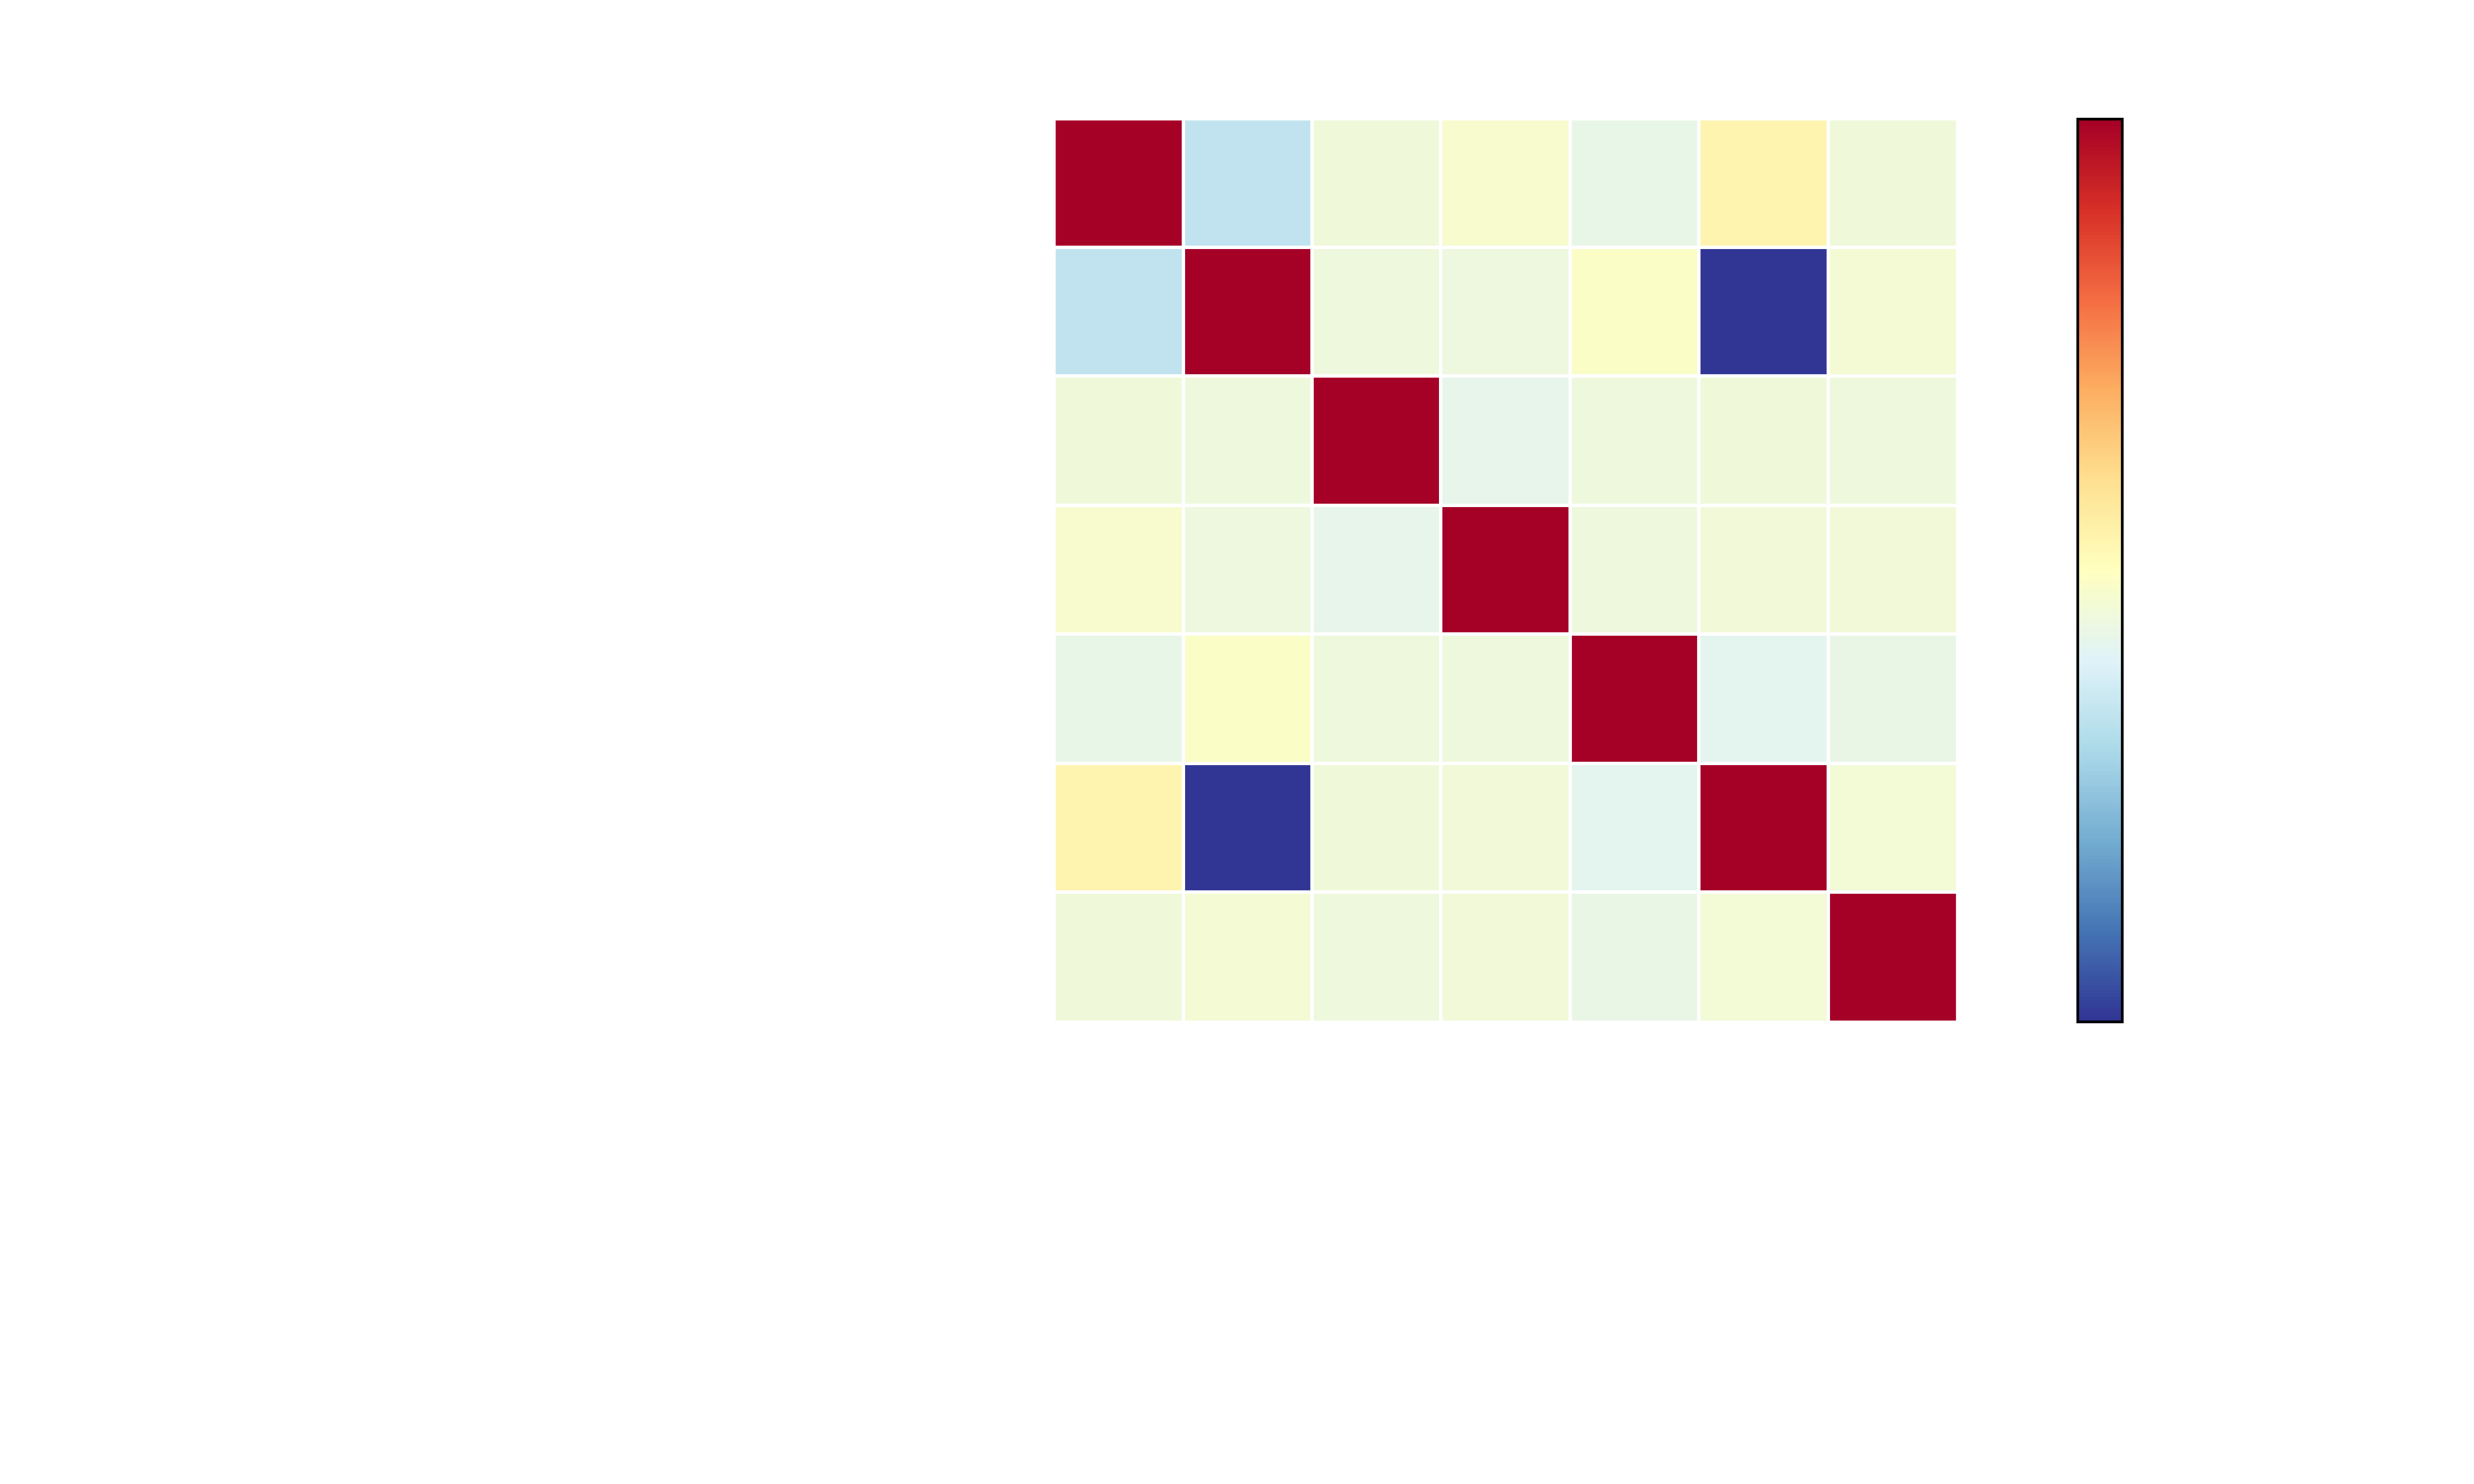
\includegraphics[width=\textwidth]{../figs/model5_corr_matrix.png}}
    \caption{\label{fig:corr_matrix_model5} Correlation Matrix - Candidate Model}
\end{figure}
\vskip 1cm

\section{Model Selection}

\indent Our key observation during model selection arose in differentiating the preformance of Fisher's linear discriminant and binary logistic regression.  While both procedures are common choices for two-level classification, and often yield simiar results, there aa few critical assumptions that differ between them.  The linear discriminant analysis (LDA) mandates the within-group covariance between each level of the endogenous variable be equal.  Additionally, the LDA model is susceptible to the influence of extreme observations, and will potentially yield inconsistent results when outliers are not accounted for.  Conversely, the logarithmic analysis has no exigence on the form of the model's predictors.  The prevalence of outliers in the dataset, exposed during the exploratory analysis, was sufficient enough cause to move forward with the logistic regression as a conservative base on which we could build our predictions. Beta models using LDA can be found in the appendix (\ref{appendix-a}).



\indent Several iterations of model selection concluded on a final model that yielded a 0.615 AUC, with exceptional sensitivity (true positive rate) and moderate specificity (true negative rate). (table \ref{tbl:modelsummary}). Categorical predictors in the final model were substituted for dummied predictors for estimate. (See regression formula - \ref{eq:1})
\vskip 1cm
\begin{table}[!ht]
    \centering
    \begin{tabular}{ll}
    \multicolumn{2}{c}{\textbf{Model 5}} \\
    Log Loss            & 0.6664         \\
    AUC                 & 0.6155         \\
    Sensitivity         & 0.744          \\
    Specificity         & 0.425
    \end{tabular}
    \end{table}
    \captionof{table}{Logistic Model Summary}\label{tbl:modelsummary}
    \bigbreak



\vskip 1cm

\begin{align}
    \resizebox{.9 \textwidth}{!} {
    \begin{aligned}
    Logit(\frac{\pi}{1-\pi}) & = \beta_0 + \beta_1\text{shot\_distance} + \beta_2\text{playoffs}_0 + \beta_3\text{playoffs}_1 + \beta_4\text{arena\_temp} + \beta_5\text{game\_event\_id} + \beta_6\text{lat} + \beta_7\text{lon} \\
    \\
    &\text{Regular Season (playoffs = 0)} \\
    & = \beta_0 + \beta_1\text{shot\_distance} + \beta_2(1) + \beta_3(0) + \beta_4\text{arena\_temp} + \beta_5\text{game\_event\_id} + \beta_6\text{lat} + \beta_7\text{lon} \\
    & = \beta_0 + \beta_1\text{shot\_distance} + \beta_2 + \beta_4\text{arena\_temp} + \beta_5\text{game\_event\_id} + \beta_6\text{lat} + \beta_7\text{lon} \\\\
    Logit(\frac{\pi}{1-\pi})& = \beta_0 + \beta_1x_1 + \beta_2x_2 + \beta_4x_4 + \beta_5x_5 + \beta_6x_6 + \beta_7x_7
    \\\\
    &\text{Playoffs (playoffs = 1)} \\
    & = \beta_0 + \beta_1\text{shot\_distance} + \beta_2(0) + \beta_3(1) + \beta_4\text{arena\_temp} + \beta_5\text{game\_event\_id} + \beta_6\text{lat} + \beta_7\text{lon} \\
    & = \beta_0 + \beta_1\text{shot\_distance} + \beta_3 + \beta_4\text{arena\_temp} + \beta_5\text{game\_event\_id} + \beta_6\text{lat} + \beta_7\text{lon} \\\\
    Logit(\frac{\pi}{1-\pi})& = \beta_0 + \beta_1x_1 + \beta_3x_3 + \beta_4x_4 + \beta_5x_5 + \beta_6x_6 + \beta_7x_7
    \end{aligned}
    }
\end{align}
\label{eq:1}

\vskip 1cm

A model composition chart, displayed in figure \ref{fig:model5features} shows the features selected in the champion model, along with the model's confusion matrix.

\begin{figure}[!hb]
    \center{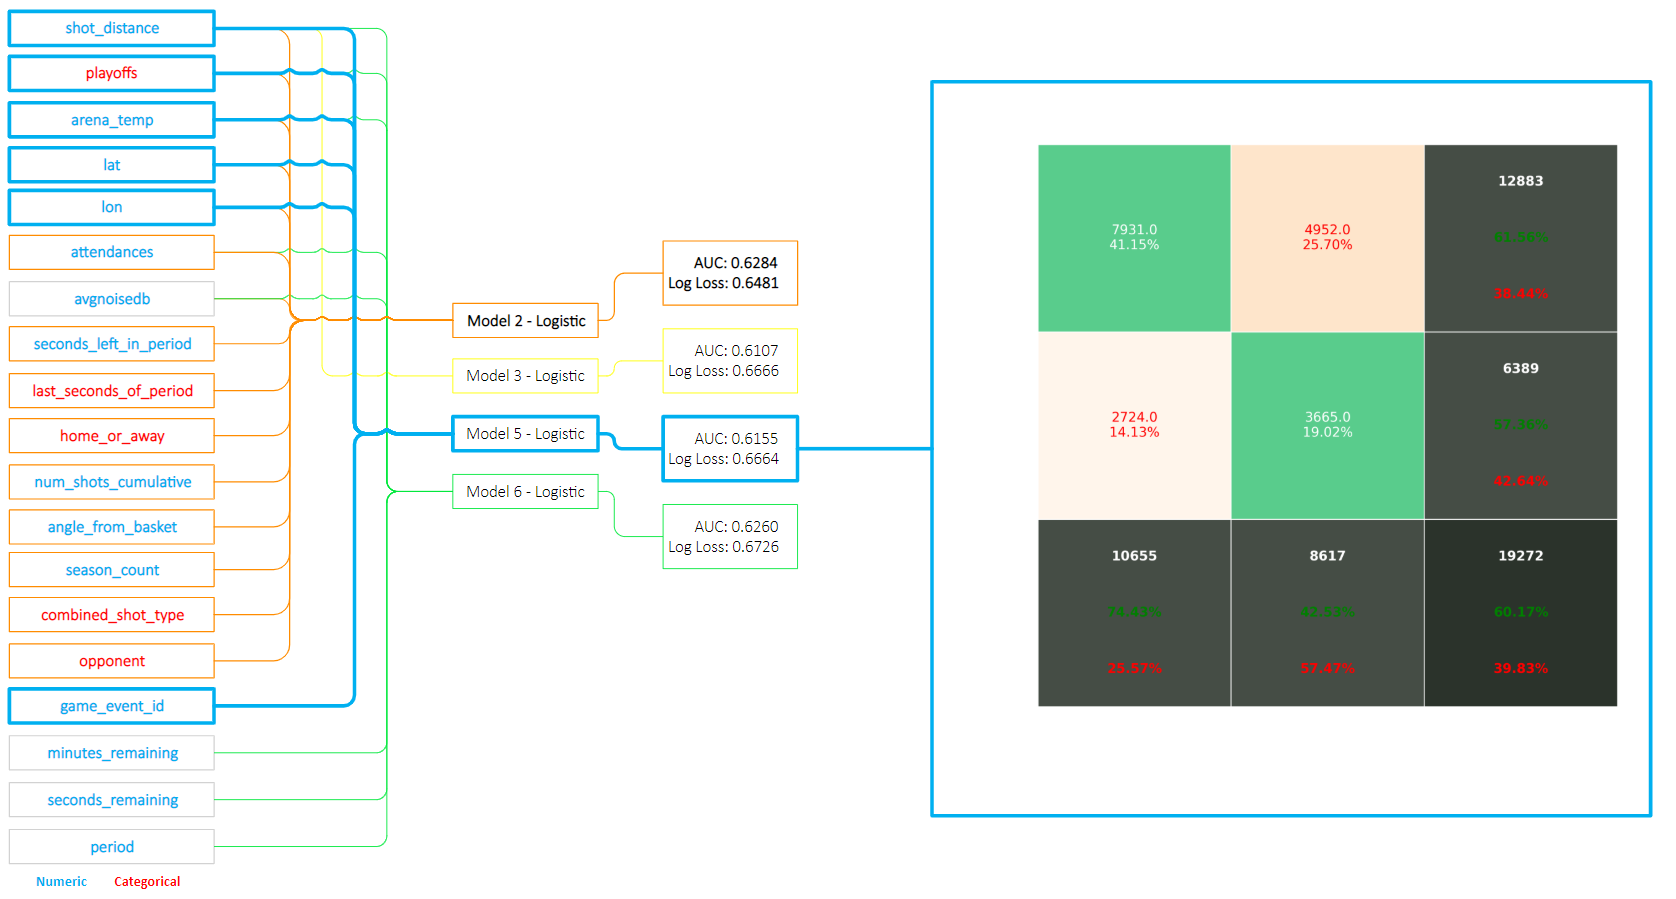
\includegraphics[width=\textwidth]{../figs/model5features.PNG}}
    \caption{\label{fig:model5features} Model Composition Chart}
\end{figure}
\cite{cm}

A full listing of candidate models can be seen in the appendix (\ref{appendix-a}).

\section{Evaluation}
\vskip 1cm
Goodness of fit measured by logarithmic loss function, where: $$ Log Loss = -(y\,log(p) + (1 - y)log(1 - p)) $$
\vskip 1cm
\indent Logarithmic loss (related to cross-entropy) measures the performance of a classification model where the prediction input is a probability value between 0 and 1. Log Loss takes into account the uncertainty of a prediction based on how much it varies from the actual label, insead of simply counting if the predicted value exactly equals the true value, as is the case with accuracy. This gave us a more nuanced view into the performance of our model.